\section{ساخت فایل خروجی اکسل در سیف\label{sec:prepare-safe}}
مراحلی که در زیر آمده است برای آماده سازی فایل نرم افزار برش پانچ کفایت میکند. بنابراین نیاز به انجام کار اضافی نیست. مثلا نیاز به تخصیص سختی خاک، المانهای ستون
\lr{(Stiff)}
و ... نمی باشد.


\subsection{ترسیم هندسه پی}
در این مرحله فقط هندسه پی مطابق شکل 
\ref{geometry}
ترسیم می شود. سعی کنید در این مرحله تمیزکاری زیادی نکنید. منظورم این هست که 
\textbf{هم پوشانی}
 نوارهای فنداسیون چه در سیف و چه در نرم افزار برش پانچ مشکلی ایجاد نمیکند،
بنابراین سعی نکنید که لبه های نوارها را بهم بچسبانید، بلکه اجازه دهید مقداری هم پوشانی در نوارها ایجاد شود.
برای ترسیم پی های نواری میتوانید از 
\textbf{بازشو}
 هم استفاده کنید و نرم افزار برش پانچ با ترسیم بازشو مشکلی ندارد و محاسبات پانچ به درستی انجام میگیرد.

\begin{figure}[H]
    \centering
    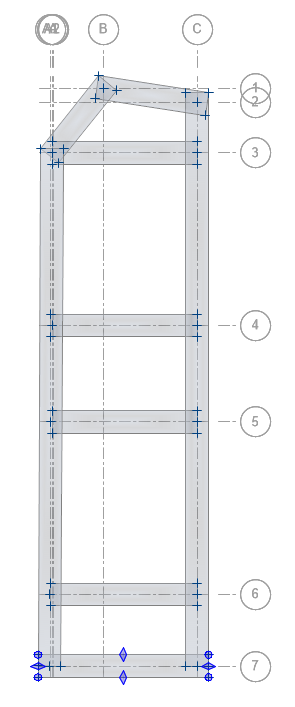
\includegraphics[scale=.6]{figures/geometry2}
    \caption{ترسیم هندسه پی در سیف}
    \label{geometry}
\end{figure}


\subsection{اختصاص مقطع به پی}
در این مرحله از منوی 
$Assign \rightarrow Slab Data \rightarrow Properties$
به هندسه ترسیم شده مقطع مناسب را اختصاص دهید (شکل 
\ref{assign}):

\begin{figure}[H]
    \centering
    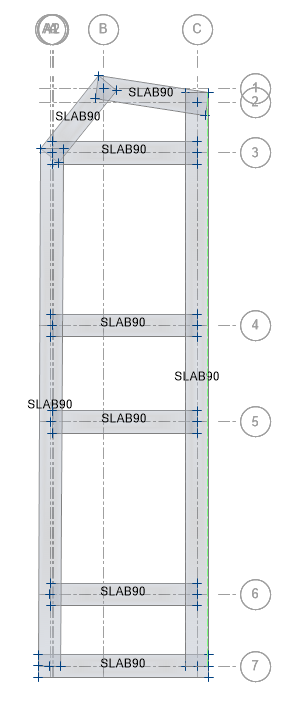
\includegraphics[scale=.6]{figures/assign}
    \caption{اختصاص مقطع به پی}
    \label{assign}
\end{figure}


\subsection{خروجی به اکسل}
مطابق شکل 
\ref{excel}
از منوی 
$File \rightarrow Export Model \rightarrow Excel $
خروجی به اکسل را انتخاب کنید. مطابق شکل 
\ref{excel2}
تیک بخش
\lr{MODEL DEFINITION}
را بزنید و 
در قسمت 
\lr{Select Load Patterns}
تمامی الگوی بارها را انتخاب و واحد خروجی را 
$KN, mm, C$
برگزینید. فایل را در محل دلخواه ذخیره کنید.

\begin{figure}[H]
    \centering
    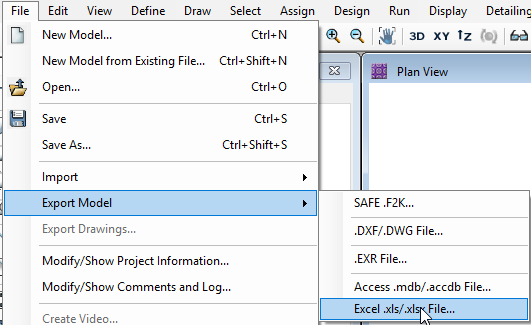
\includegraphics[width=.7\linewidth]{figures/excel}
    \caption{خروجی به اکسل}
    \label{excel}
\end{figure}

\begin{figure}[H]
    \centering
    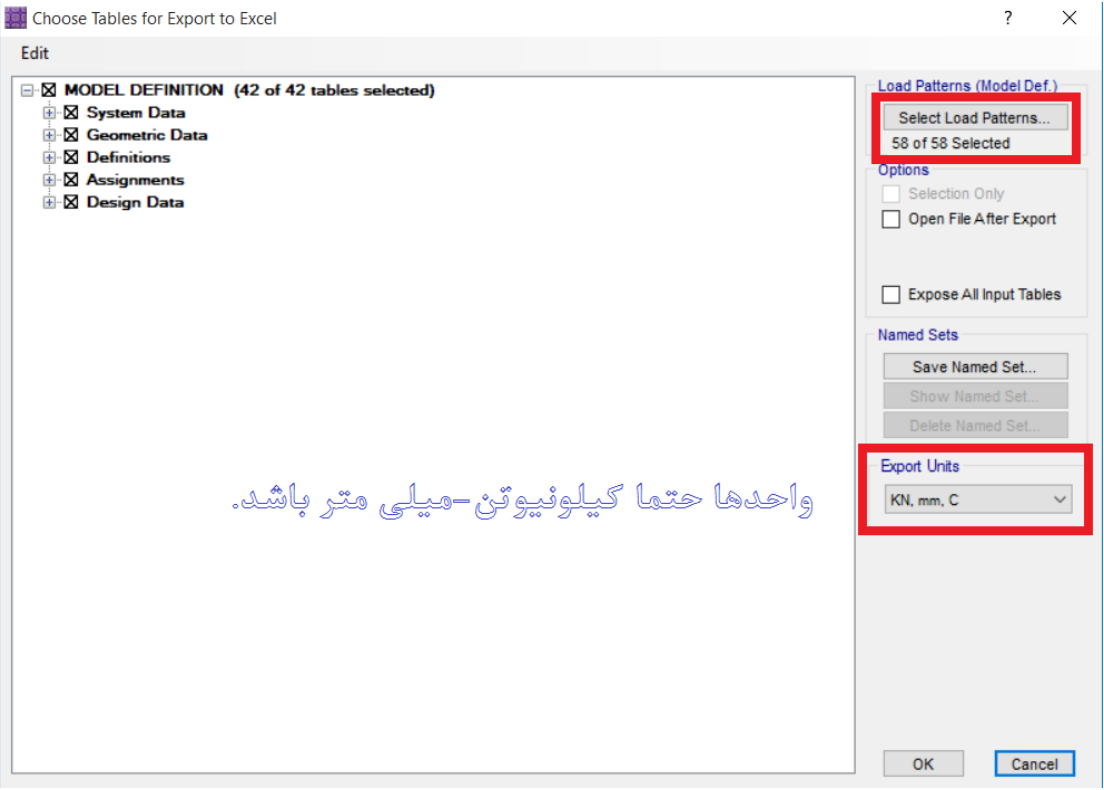
\includegraphics[width=.7\linewidth]{figures/excel2}
    \caption{تنظیم پارامترهای خروجی فایل اکسل}
    \label{excel2}
\end{figure}